\documentclass[oneside]{book}
\author{Matt Caswell}
\title{Developing Applications with OpenSSL}
\usepackage{color}
\usepackage{colortbl}
\usepackage{graphicx}
\usepackage{listings}
\usepackage{xcolor}
\newcommand\todo[1]{\textcolor{red}{[TODO:#1]}}
\definecolor{LightGray}{gray}{0.9}
\lstdefinestyle{osslc}{
  breaklines=true,
  frame=single,
  xleftmargin=\parindent,
  language=C,
  showstringspaces=false,
  basicstyle=\footnotesize\ttfamily,
  numbers=left,
  numberstyle=\tiny,
  captionpos=b
}
\begin{document}
\lstset{style=osslc}
\maketitle
\tableofcontents
\part{Introduction}
\chapter{About OpenSSL}
Add some text here.

\part{SSL/TLS/DTLS Application Programming}
\chapter{Understanding SSL/TLS}
Let's start off with some basics and a bit of history. SSL is the ``Secure 
Sockets Layer'' and was first developed by Netscape Communications. Later the 
protocol was standardised by the IETF\footnote{The Internet Engineering Task 
Force or IETF, is an organisation that publishes many of the standards relevant 
to SSL/TLS. The standards are published in the form of documents known as RFCs. 
The most significant of these from our perspective are RFC6101 (SSL3.0), 
RFC2246 (TLS1.0), RFC4346 (TLS1.1) and RFC5246 (TLS1.2)} and was renamed to TLS 
(Transport Layer Security).

The purpose of SSL/TLS is to secure the communications between two parties. The
initiating  party is known as the ``client'' and the responding party is known
as the ``server''. The term ``secure'' here covers authentication,
confidentiality and integrity. In other words an attacker should not be able 
to:
\begin{itemize}
\item fool a party into believing that they are someone else;
\item eavesdrop and hence learn the content of messages being exchanged; or
\item modify those messages without being detected.
\end{itemize}

There are limits to the security that is provided by the protocol; for example
there is no  provision for preventing an attacker from learning that two parties
are engaging in communications and their associated IP addresses. Nor does it
prevent an attacker from learning the approximate size of messages transferred.

There are multiple versions of SSL/TLS:
\begin{itemize}
\item SSL 1.0. This version was developed by Netscape but was never publicly 
released due to fundamental security flaws.
\item SSL 2.0. This was the first publicly released version of the protocol. It 
was first published in February 1995, but is no longer in common usage due to 
significant security issues. OpenSSL 1.1.0 no longer supports this version.
\item SSL 3.0. This was the last version of the protocol developed by Netscape 
and represented a significant change from version 2.0. All subsequent versions 
were based on this version. It should no longer be used although there are 
still some servers on the internet which only support this version.
\item TLS 1.0. The first version of the protocol published by the IETF. In 
practice this is very similar to SSL 3.0, although one of the major differences 
is the support for \emph{extensions}.
\item TLS 1.1. Published in 2006 this provided a number of security tweaks.
\item TLS 1.2. Published in 2008 this version provided some significant changes
including  support for authenticated encryption ciphers.
\end{itemize}

The protocol provides the capability for the two parties to negotiate between 
them which version of the protocol will be used. For example if the client 
supports all versions up to TLS 1.2, but the server only supports versions up 
to TLS 1.0, then version negotiation will take place and agree on the highest 
available version that both support (in this case TLS 1.0).

\section{Establishing Identity}

In order to authenticate a remote party there has to be a system in place for 
reliably establishing and verifying the identify of that party. Most commonly 
SSL/TLS only authenticates the server not the client, i.e. from a server's 
perspective the identity of the client is unknown, but the client is able to 
confirm that they are talking to the server that they think they are (and not a 
malicious attacker pretending to be that server). Frequently higher level 
application protocols may add the capability to authenticate clients, although
it is also possible to do it at the SSL/TLS layer if so desired.

Identity is established through the use of a \emph{digital certificate}. The 
digital certificate provides public data about a server for which it is issued. 
For example, the certificate will contain the hostname(s) for which it is 
valid. In order to obtain a certificate a server operator must first create a 
private and a public key. The private key must remain secret. Loss of the 
private key would be catastrophic to the security of the system. Anyone with 
access to the private key can masquerade as the server. The public key is 
mathematically related to the private key, although it is not possible to 
derive the private key from it. The public key is published in the digital 
certificate and it is safe for this to be available to everyone.

Having obtained a private/public key pair a server operator must obtain their
certificate from a \emph{Certificate Authority} (CA)\footnote{CAs can be
privately run and purely internal to an organisation; or they could be public.
Which type is most appropriate will depend on what the certificte will be used
for. There are many public CAs available. A simple search in your search engine
of choice should turn up lots of links. Many, but not all, charge a fee for
issuing a certificate.}. The CA will, at a minimum, verify that the server 
operator is in control of the domain name to be included in the certificate. 
Dependant on the type of certificate ordered, other checks may also be 
performed to verify the identity of the server operator. Finally the CA will 
issue the certificate which itself will be digitally signed by the CA.

Both the digital certificate, and the associated private key are installed on 
the SSL/TLS server. When a client accesses the server, the server will send 
its certificate back to the client. In order for authentication to be
successful the client must verify two things:
\begin{enumerate}
\item The certificate provided by the server is valid and issued by a CA that 
the client trusts.
\item The server has the private key corresponding to the public key published 
in the certificate.
\end{enumerate}

Part of the role of the SSL/TLS protocol is to enable the client to perform the 
above checks during the establishment of a connection. If either of these 
checks fail then the connection will fail.

As mentioned above it is also possible for the server to authenticate the 
client as part of the SSL/TLS protocol. If this capability is used then it works
in a very similar way  to that described above. The primary difference is that
the client will also have to create a private/public key pair and obtain a
digital certificate from a CA that the server trusts. 

\section{Ciphersuites}

SSL/TLS itself does not mandate the use of any particular cryptographic 
algorithms. Instead it provides a framework for combining different algorithms 
together and enabling the client and server to negotiate between them which 
combination of algorithms will be used to protect messages that are exchanged. 
A group of algorithms combined in this way is known as a \emph{ciphersuite}. 
There are many different ciphersuites that are available\footnote{At the time 
of writing OpenSSL 1.1.0 supports 168 different ciphersuites}. Each
ciphersuite identifies a set of algorithms that it will use to satsify the 
following cryptographic primitives:
\begin{itemize}
\item Authentication. What algorithm will be used to digitally sign various 
aspects of the communication in order to establish and verify the identify of
the parties (either just the server, or both the server and the client). The 
algorithm used here will be the same one used to generate the public/private 
key pair associated with the digital certificate. Examples of common algorithms 
include RSA, DSA and ECDSA.
\item Key Exchange. Typically a new encryption key will be generated for each
connection. Do not confuse this encryption key with the public/private key pair
associated with the digital certificate. The encryption key must be shared
between both ends of the communication and must be \emph{private} to prevent an
eavesdropper from being able to decrypt messages. Key exchange algorithms solve 
the problem of how two parties will agree on a key without enabling an 
eavedropper to work out what it is. Examples of algorithms that are used for 
this purpose include RSA, DH and ECDH.\footnote{You will also very
frequently come across the so-called ``ephemeral'' variants of DH and ECDH
known as DHE and ECHDE respectively.}
\item Encryption. Having established a shared encryption key, the two 
communicating parties can start to protect their communications from 
eavesdroppers by encrypting the data that they exchange. Examples of common 
encryption algorithms include AES, CAMELLIA and ChaCha20.
\item Integrity. The algorithm used to protect communications from being 
tampered with by an attacker. Often the algorithm used here will be one known 
as HMAC combined with a message digest algorithm such as SHA256 or SHA512. A
message digest is simply a secure ``hash'' function. They take arbitrary 
length input data and output a fixed length ``hash'' value that exhibits 
certain security properties (including that it is not possible to derive the 
input data from the hash output). Alternatively, integrity could be provided by
a \emph{mode} of the underlying  encryption cipher. Modes are a complex topic,
but in essence define the manner in which an encryption algorithm is used.
Examples of modes that provide integrity include GCM and CCM.
\end{itemize}

To look at some example ciphersuites you can use the \lstinline!openssl ciphers!
command line tool:
\begin{verbatim}
$ openssl ciphers -v
\end{verbatim}

The \lstinline!-v! argument here instructs OpenSSL to display verbose output.
Without any other arguments this will list information about the DEFAULT
ciphersuites (i.e. those ciphersuites that are available unless you configure
OpenSSL differently).

\begin{lstlisting}[float=tb,label=lst:ciphers-extract,caption=An
extract from \lstinline!openssl ciphers -v! output]
ECDHE-ECDSA-AES256-GCM-SHA384 TLSv1.2 Kx=ECDH     Au=ECDSA Enc=AESGCM(256) Mac=AEAD
ECDHE-RSA-AES256-GCM-SHA384 TLSv1.2 Kx=ECDH     Au=RSA  Enc=AESGCM(256) Mac=AEAD
DHE-RSA-AES256-GCM-SHA384 TLSv1.2 Kx=DH       Au=RSA  Enc=AESGCM(256) Mac=AEAD
ECDHE-ECDSA-CHACHA20-POLY1305 TLSv1.2 Kx=ECDH     Au=ECDSA Enc=CHACHA20/POLY1305(256) Mac=AEAD
ECDHE-RSA-CHACHA20-POLY1305 TLSv1.2 Kx=ECDH     Au=RSA  Enc=CHACHA20/POLY1305(256) Mac=AEAD
DHE-RSA-CHACHA20-POLY1305 TLSv1.2 Kx=DH       Au=RSA  Enc=CHACHA20/POLY1305(256) Mac=AEAD
ECDHE-ECDSA-AES128-GCM-SHA256 TLSv1.2 Kx=ECDH     Au=ECDSA Enc=AESGCM(128) Mac=AEAD
ECDHE-RSA-AES128-GCM-SHA256 TLSv1.2 Kx=ECDH     Au=RSA  Enc=AESGCM(128) Mac=AEAD
DHE-RSA-AES128-GCM-SHA256 TLSv1.2 Kx=DH       Au=RSA  Enc=AESGCM(128) Mac=AEAD
ECDHE-ECDSA-AES256-SHA384 TLSv1.2 Kx=ECDH     Au=ECDSA Enc=AES(256)  Mac=SHA384
ECDHE-RSA-AES256-SHA384 TLSv1.2 Kx=ECDH     Au=RSA  Enc=AES(256)  Mac=SHA384
DHE-RSA-AES256-SHA256   TLSv1.2 Kx=DH       Au=RSA  Enc=AES(256)  Mac=SHA256
ECDHE-ECDSA-AES128-SHA256 TLSv1.2 Kx=ECDH     Au=ECDSA Enc=AES(128)  Mac=SHA256
ECDHE-RSA-AES128-SHA256 TLSv1.2 Kx=ECDH     Au=RSA  Enc=AES(128)  Mac=SHA256
DHE-RSA-AES128-SHA256   TLSv1.2 Kx=DH       Au=RSA  Enc=AES(128)  Mac=SHA256
ECDHE-ECDSA-AES256-SHA  TLSv1 Kx=ECDH     Au=ECDSA Enc=AES(256)  Mac=SHA1
ECDHE-RSA-AES256-SHA    TLSv1 Kx=ECDH     Au=RSA  Enc=AES(256)  Mac=SHA1
\end{lstlisting}

An extract of the output from \lstinline!openssl ciphers -v! is given in 
Listing \ref{lst:ciphers-extract}. The columns tell you the following
information:
\begin{itemize}
\item The ciphersuite name such as \lstinline!ECDHE-ECDSA-AES256-CCM8!.
\item The earliest protcol version that the ciphersuite is available from. Note 
that ciphersuites are \emph{forward compatible}. Therefore if a ciphersuite is
marked as \lstinline!SSLv3! then it is compatible with all protocol versions 
from SSL 3.0 right up to TLS 1.2.
\item The key exchange algorithm used by the ciphersuite (\lstinline!Kx! here 
stands for ``Key Exchange'').
\item The algorithm being used to provide authentication (\lstinline!Au!).
\item The encryption (\lstinline!Enc!) algorithm.
\item The algorithm being used to provide integrity. This will either be a 
message digest that is being used in conjunction with the HMAC algorithm, or it
will indicate that integrity is being provided by a mode of the encryption 
cipher (\lstinline!AEAD!).
\end{itemize}

\section{Records}

Data is transferred between clients and servers using \emph{records}. Think of 
a record as being like an envelope containing data. The envelope has some basic 
information about its contents written on it, such as:
\begin{itemize}
\item The amount of data that is being transferred
\item The type of data that is being transferred
\end{itemize}

The record will also apply any cryptographic operations to the data that may be 
appropriate dependant on the current state of the connection. During initial 
connection various parameters need to be agreed between the two parties to 
determine exactly what cryptographic operations will be applied. One of these 
parameters is the ciphersuite. The ciphersuite that is currently in use will 
define the encryption that is to be applied to the data within the record.

As well as the encrypted data the record will also contain a Message 
Authentication Code (MAC). The MAC utilises the integrity algorithm and a 
secret key, shared between the two parties, to calculate a code that is unique
to the data being sent. Any attempt by an attacker to modify the data will mean
that the MAC code will fail to verify when it is checked by the remote party 
and the connection will be aborted.

Optionally records can also compress the data that they transmit. This is done 
prior to encryption. This is usually not done in practice due to security 
concerns associated with this capability.

\section{The Handshake}

The initial exchange of messages during which cryptographic parameters are 
exchanged is known as the \emph{handshake}. While making the initial connection
no crypotgraphic parameters will have yet been agreed. Therefore there is no
encryption and no MAC on individual records.  Record data is sent in
\emph{plaintext}. For this reason the protocol has been designed such that no
application data is sent until the connection has been established and
cryptographic parameters have been agreed. A MAC of the entire set of handshake 
messages is calculated and verified at the last step of the handshake process. 
In this way, even though inidividual records do not have integrity protection, 
the handshake as a whole does.

Handshake messages are transmitted between the client and server in rec-ords. A 
single record may contain multiple handshake messages, or a single handshake 
message may be spread across multiple records. A handshake is always initiated 
by a client sending a ``ClientHello'' message to a server. A typical handshake 
is shown in figure \ref{fig:typical-hand}.

\begin{figure}[t]
\fbox{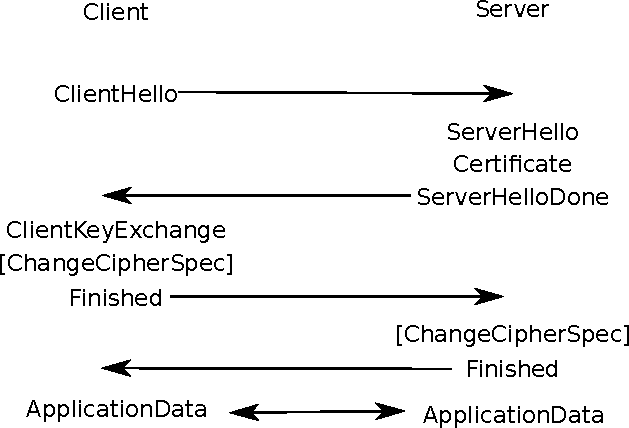
\includegraphics[width=0.9\textwidth]{devel-tls/understand-tls/typicalhand.pdf}}
\caption{A typical SSL/TLS handshake.}
\label{fig:typical-hand}
\end{figure}

The ClientHello contains:
\begin{itemize}
\item The highest protocol version supported by the client.
\item Some random data generated by the client.
\item The id of a pre-existing session that the client wishes to use (if any).
\item A list of the ciphersuites the client is willing to use.
\item A list of the compression methods the client is willing to use (if any).
\item A list of \emph{extensions} the client supports.
\end{itemize}

There are quite a few different messages possible and not all messages will 
always be sent. Some messages are optional and may depend on the ciphersuite 
chosen; whether the client is required to provide a certificate; etc. The 
handshake shown in figure \ref{fig:typical-hand} is an example of a full 
handshake. Once a client has completed its first handshake with a server it can 
usually reuse the cryptographic parameters negotiated so that it does not need 
to go through a second or subsequent full handshake. Instead it performs an 
\emph{abbreviated handshake} and reuses the previously negotiated parameters. 
This is called \emph{session resumption}. A server may refuse to resume a 
session (for example if the session on the server has expired), in which case a 
full handshake will occur.

\chapter{Getting started}
This chapter will cover some of the most basic things that you need to 
understand in order to write some very simple SSL/TLS code. Let's start off with
a ``Hello World'' client. It's purpose is simply to open up an SSL/TLS
connection to a remote server, send a simple message, and then close the
connection. Don't worry if you don't understand all of the individual steps yet,
we will cover them in the rest of this chapter. See Listing
\ref{lst:hello-world-client}.

\lstinputlisting[float=p,label=lst:hello-world-client,lastline=61,
caption=A simple ``Hello World'' client]
{devel-tls/get-start/simpleclient.c}

\section{Library Initialisation}
\label{sec:getstart-library-init}

Let's walk through this code sample step-by-step. Firstly we initialise 
``libssl''. OpenSSL provides two libraries ``libcrypto'' and ``libssl''. The 
former provides all of the underlying cryptography capabilities that are 
required, as well as other ``helper'' functions. The latter adds onto that an
understanding of how to communicate using the SSL/TLS protocol. Before you can 
use libssl you must first initialise it. This initialisation step will take all 
of the necessary steps to initialise the underlying libcrypto library. However 
it only initialises ``enough'' for libssl use. Therefore if you want to 
additionally use libcrypto capabilities directly then you will need to 
explicitly initialise that too.

There are two steps to libssl initialisation. The first of these is to call 
\verb!SSL_load_error_strings()!. There are numerous errors that may occur 
during libssl usage. Some examples of errors that could occur are:
\begin{itemize}
\item A remote peer sends an illegal message.
\item It is not possible to find a ciphersuite that is acceptable to both 
parties.
\item It is not possible to find a common protocol version. 
\item The remote peer unexpectedly closed the connection.
\item Some internal error (bug) was hit.
\end{itemize}

OpenSSL maintains an internal table of all the errors that could occur along 
with their human readable description, as well as the internal function and 
line number within the library that issued the error. This information is very 
helpful for tracking down problems. For this reason calling 
\verb!SSL_load_error_strings()! is strongly recommended before using 
libssl. The disadvantage is that loading this table of data does consume some 
memory. This could be a problem in some environments (e.g. embedded systems), 
and therefore in certain circumstances you may be appropriate to not load the
error strings. If you choose to omit this step though, be prepared for later 
difficulties in the event that errors occur.

The second step in initialisation is to call \verb!SSL_library_init()!. 
This performs a number of initialisation steps including preparing the required 
ciphers and digests for use. Calling this function is mandatory prior to 
calling other libssl functions. You may encounter references to two other 
functions in some sources:
\begin{itemize}
\item\verb!OpenSSL_add_ssl_algorithms()!; and 
\item\verb!SSLeay_add_ssl_algorithms()!.
\end{itemize}
These two functions are actually  synonyms for \verb!SSL_library_init()! but are
present for backwards compatibility reasons only, i.e. don't use them in new
code.

\section{Creating an \texttt{SSL\_CTX}}

In order to create an SSL/TLS connection you must first create an
\verb!SSL_CTX! object. A single \verb!SSL_CTX! can be shared across
many SSL/TLS connections. It provides a mechanism for setting up configuration
that is common to a set of connections. Creating an \verb!SSL_CTX! is 
simply a matter of calling the function \verb!SSL_CTX_new!. That function 
takes an \verb!SSL_METHOD! as a parameter. For clients there are five 
primary \verb!SSL_METHOD!s that could be used:
\begin{itemize}
\item \verb!SSLv3_client_method()! Connections based on this method are 
\emph{only} capable of using SSLv3.0.
\item \verb!TLSv1_client_method()! Creates connections that can 
\emph{only} use TLS v1.0.
\item \verb!TLSv1_1_client_method()! Creates connections that can 
\emph{only} use TLS v1.1.
\item \verb!TLSv1_2_client_method()! Creates connections that can 
\emph{only} use TLS v1.2.
\item \verb!TLS_client_method()! Creates connections that can negotiate 
the highest available protocol version.
\end{itemize}

You may see references to \verb!SSLv23_client_method()!. This is the old 
name for \verb!TLS_client_method()! and is synonymous with it. New code 
should use the new name. Don't be confused by the old name - 
\verb!SSLv23_client_method()! is capable of negotiating \emph{all} 
supported protocol versions.

Normally you only ever need to use \verb!TLS_client_method()!. Don't use 
the other protocol specific methods unless you really need to. If you want to 
be able to restrict which protocol versions can be negotiated (for example to 
prevent SSLv3 from being used) then there are a set of options to allow this 
(see table \ref{tab:protocol-opts}).

\begin{table}[tb]
\centering
\begin{tabular}{|l|l|}
\hline
\rowcolor{LightGray}
Option Name & Option Description \\
\hline
\verb!SSL_OP_NO_SSLv3! & Disable SSL v3 support \\
\hline
\verb!SSL_OP_NO_TLSv1! & Disable TLS v1.0 support \\
\hline
\verb!SSL_OP_NO_TLSv1_1! & Disable TLS v1.1 support \\
\hline
\verb!SSL_OP_NO_TLSv1_2! & Disable TLS v1.2 support \\
\hline
\end{tabular}
\caption{Protocol negotiation options}
\label{tab:protocol-opts}
\end{table}

To apply these options you use the \verb!SSL_CTX_set_options()! command. You 
can also set them on individual \verb!SSL! objects if you wish to have that 
level of control using \verb!SSL_set_options()!. You must do so \emph{before} 
any connection is established in order for them to have an effect. You can 
``OR'' multiple options together if you want to disable multiple options in one 
go. For example the following code disables both SSL v3 and TLS v1.0:
\begin{lstlisting}
SSL_CTX_set_options(SSL_OP_NO_SSLv3 | SSL_OP_NO_TLSv1);
\end{lstlisting}

You should only have a single contiguous range of enabled protocol versions, 
e.g. do not disable SSL v3 and TLS v1.1, whilst keeping TLS v1.0 and TLS v1.2 
enabled.

In our simple client code in listing \ref{lst:hello-world-client} we are not
disabling any protocol versions so we simply call \verb!SSL_CTX_new()! with
\verb!TLS_client_method()!. The \verb!SSL_CTX_new! function will return a
\verb!NULL! result if something went wrong, so it is important that you check
the return value.

In our example code we are also specifying an additional setting for our
\verb!SSL_CTX! through a call to \verb!SSL_CTX_set_verify()!. This defines the 
behaviour we want for verifying any digital certificates that servers might
present to us. This function actually provides us with the capability to define 
a very fine degree of control over that verification process. It takes three 
arguments:
\begin{enumerate}
\item a pointer to the \texttt!SSL\_CTX! that we are working with;
\item a verification mode that we wish to apply to the \texttt!SSL\_CTX!; and
\item an optional callback function.
\end{enumerate}

For clients the verification mode that you almost always want to set is 
\verb!SSL_VERIFY_PEER!. This causes OpenSSL to verify the certificate that the 
server presents to us, and abort the connection if that verification fails. You
should \emph{always} set this for clients unless you really know what you are 
doing.

In our example we are not going to use the callback function, so we just set 
that to \verb!NULL!.

\section {Connecting to a server}

Having set up our \verb!SSL_CTX! object, the next step is to connect to a
server.  Before we can do that though we need to set up a server that we can
use.  Fortunately openssl provides a test server for that purpose. However,
before we  can use it, we need to create a certificate an private/public key
pair.

\subsection {Creating a self-signed certificate}

We are going to create a new certificate for our test server which will be 
``self-signed''. With a normal certificate a private/public key pair is
generated and then the public key is published as part of the certificate, 
which is then signed using the private key of the \emph{CA}. In a self-signed 
certificate a CA is not used, but instead the certificate is signed by the 
private key which is the pair of the public key in the certificate itself! 
Self-signed certificates have the advantage that they are easy to produce 
because you do not have to go through an external CA to get one. The 
disadvantage is that you (usually) cannot use them on public servers because 
they will not be trusted by clients. For our purposes a self-signed certificate 
will be sufficient.

First we create our private key. The algorithm we are going to use is  RSA with
a key length of 2048 bits. The key can be created using the OpenSSL command line
tool. The following command generates the key and stores it in the file 
``server.key'':
\begin{verbatim}
openssl genrsa -out server.key 2048
\end{verbatim}

Note that in this example we are not encrypting the private key and securing it 
with a password. For a real key you might wish to do that (e.g. by using the 
\verb!-aes128! argument).

Next we need to create a ``Certificate Signing Request'' (CSR). Typically this 
is a file that is created for sending to a CA. However in this case we will use 
it to create our self-signed certificate. The CSR generation process collects 
together all of the information that you are requesting that the CA includes in 
the certificate. Note that just because you have included something in a CSR 
does not mean that the CA is obliged to include it in the certificate. We 
create the CSR by using the OpenSSL \verb!req! command line tool. This will ask 
a number of questions about the organisation that we are creating the CSR for. 
The most important field here is the ``Common Name''. This should be set to the 
fully qualified domain name for the server. Our test server is only going to be 
used on our local machine, so we set this to 127.0.0.1. The following command 
stores the CSR in the file ``server.csr'':

\begin{verbatim}
$ openssl req -new -key server.key -out server.csr
You are about to be asked to enter information that will be inco\
rporated
into your certificate request.
What you are about to enter is what is called a Distinguished Na\
me or a DN.
There are quite a few fields but you can leave some blank
For some fields there will be a default value,
If you enter '.', the field will be left blank.
-----
Country Name (2 letter code) [AU]:UK
State or Province Name (full name) [Some-State]:Derbyshire
Locality Name (eg, city) []:
Organization Name (eg, company) [Internet Widgits Pty Ltd]:Test
Organizational Unit Name (eg, section) []:
Common Name (e.g. server FQDN or YOUR name) []:127.0.0.1
Email Address []:

Please enter the following 'extra' attributes
to be sent with your certificate request
A challenge password []:
An optional company name []:
\end{verbatim}

The final step is to generate the certificate based on the information 
contained with the CSR file, and sign it with the private key that we generated 
in the first step.

\begin{verbatim}
$ openssl x509 -req -days 365 -in server.csr \
               -signkey server.key -out server.pem
\end{verbatim}

This command creates a certificate with a validity period of 365 days and 
stores it in the file ``server.pem''.

\subsection{Starting the test server}
\label{sec:start-test-server}

Now that we have created our self-signed certificate we can start up our test 
server:

\begin{verbatim}
$ openssl s_server -key server.key -cert server.pem -accept 1443
Using default temp DH parameters
ACCEPT
\end{verbatim}

\subsection{The client connection code}

In order to connect to a server from our code we first need to create a standard
TCP connection. We used a helper function to do this in listing
\ref{lst:hello-world-client} - \verb!create_tcp_connection()!. This takes two
arguments: the IP address of the server to connect to; and the port number. This
helper function is shown in listing \ref{lst:create-tcp-connection}. There is 
nothing OpenSSL specific about how this works.

\lstinputlisting[float=tb,label=lst:create-tcp-connection,firstline=63,
caption=The \texttt{create\_tcp\_connection()} function]
{devel-tls/get-start/simpleclient.c}

Assuming this works successfully, the next step is to create our \verb!SSL! 
object via a call to \verb!SSL_new!. This takes as an argument the 
\verb!SSL_CTX! that we created earlier, and thus inherits any configuration 
settings that we applied to it (such as the method to use, and the verification 
settings). Once we have our \verb!SSL! object we then associate it with the 
underlying TCP connection using \verb!SSL_set_fd()!.

Now we have an \verb!SSL! object associated with an open TCP connection to the 
server - but we have still not initiated the SSL/TLS handshake. Before we do so 
there is one last thing that we need to set up. We have already configured (at 
the \verb!SSL_CTX! level) the verification settings, i.e. we want to verify the 
server certificate. However we have not told OpenSSL the hostname of the server 
that we expect to be in the certificate. This is a \emph{very important} 
security step. Without this OpenSSL will simply verify that the certificate
presented is valid, but will allow any hostnames. To configure this we first 
must get hold of the \verb!X509_VERIFY_PARAM!\footnote{X.509 is an ITU-T 
standard for digital certificates. There have been a number of iterations of 
the standard and we are currently on X.509v3. When we talk about a certificate 
in the SSL/TLS context we are actually referring to an X.509 certificate. 
Therefore the OpenSSL type \texttt{X509\_VERIFY\_PARAM} holds parameters for the 
verification of X.509 digital certificates} object for our SSL/TLS connection 
using \verb!SSL_get0_param()!\footnote{You will sometimes see OpenSSL APIs of 
the form \texttt{get0}, \texttt{get1}, \texttt{set0} and \texttt{set1}. This
tells you  who is responsible for ``freeing'' the memory associated with the
value that  you get or set: 0 means the application should not free it; 1 means
it should.}. Then we call \verb!X509_VERIFY_PARAM_set1_host()! and provide the 
fully qualified domain name of the server we are connecting to (in this 
example, for simplicity, we are just using an IP address). This is the domain
name that  we expect to see in the certificate presented to us. If OpenSSL
encounters a certificate with any other domain name then the connection will
fail.

The final connection step is to call \verb!SSL_connect()!. Strictly speaking
this step is optional because a handshake will be forced as soon as you attempt
to read or write to the \verb!SSL! object. However if you want to have more 
control over when the handshake occurs you can call \verb!SSL_connect! 
explicitly as shown in this example.

\section{Writing data}

Having established an SSL/TLS connection we can now start to use it. In the 
example in listing \ref{lst:hello-world-client} we simply write a single 
message to the connection using \verb!SSL_write()!. This takes three arguments:
\begin{enumerate}
\item the \texttt{SSL} object;
\item a buffer containing the data to be sent; and
\item a ``length'' parameter, i.e. the amount of data in the buffer to be sent.
\end{enumerate}

The data sent in this example is text, but \verb!SSL_write()! also supports 
sending binary data. In this example the \verb!SSL_write()! call will
\emph{block} (i.e. it will not return) until all of the data has been written
to the connection, or a fatal error has occurred. OpenSSL also supports
\emph{non-blocking} IO. See chapter \todo{Chapter reference here}.

\section{Cleaning Up}

The first step in our example clean up code in listing
\ref{lst:hello-world-client} is to print any OpenSSL errors that have been 
recorded to \verb!stderr!. Errors can occur for many reasons. There are some
examples of typical reasons in section \ref{sec:getstart-library-init}.

Next we close down the SSL connection via a call to \verb!SSL_shutdown()!. The 
purpose of this is to inform the server that we are planning on cleanly closing 
down our connection. A special message known as a ``close\_notify'' alert is 
sent. A return value of 0 from calling this function means that the client has 
sent the ``close\_notify'' but it has not yet received a ``close\_notify'' back 
from the server to acknowledge the closing down of the connection. To receive 
that we call \verb!SSL_shutdown()! a \emph{second} time.

We must also free up memory and resources allocated to our \verb!SSL! and
\verb!SSL_CTX! objects as well as our underlying TCP connection.

Finally, before application close down, we need to uninitialise libssl. In 
real applications you may need to do more uninitialisation than shown in our 
example code, dependant on what features of libssl/libcrypto you are using. For 
example you may need to uninitialise configuration modules (see chapter
\todo{ref here}); clean up engines (see chapter \todo{ref here}); or
uninitialise compression methods if you have used them (see chapter \todo{ref 
here}). 
At a minimum though you need to:
\begin{itemize}
\item Call \texttt{CRYPTO\_cleanup\_all\_ex\_data()}. Many structures within
OpenSSL have the ability to associate application specific data  (``ex\_data'')
with them. libssl itself may use this capability and therefore  this needs to be
cleaned up.
\item Remove all ciphers and digests from the internal lookup tables using 
\texttt{EVP\_cleanup()}.
\item Call \texttt{ERR\_remove\_thread\_state()} to uninitialise the thread
local error queue. Note: this function should be called for each thread in your
application.
\item Unload the human readable error strings by calling 
\texttt{ERR\_free\_strings()}.
\end{itemize}

\section {Compiling the application}

I will assume that you have already installed OpenSSL (see chapter \todo{ref 
here} if not) and that you are using shared libraries. In order to compile our 
application the compiler must be able to find the OpenSSL header files and the 
linker must be able to find the shared libraries. Dependant on how you obtained 
and installed your version of OpenSSL these may already be on the relevant 
system paths. Otherwise you have to state them explicitly. For this section I 
will assume that you are using Linux and that you have installed OpenSSL into
\verb!\usr\local\ssl!. For other Operating Systems and locations you will have 
to adjust the instructions accordingly. You can compile the application using:

\begin{verbatim}
$ gcc -o simpleclient simpleclient.c -I/usr/local/ssl/include \
      -L/usr/local/ssl/lib -lcrypto -lssl
\end{verbatim}

\section {Running the application}

To run the application first ensure that the test server is running as 
described in section \ref{sec:start-test-server}. Let's see what happens when 
we run it:

\begin{verbatim}
$ LD_LIBRARY_PATH=/usr/local/ssl/lib ./simpleclient
139770294548112:error:1416F086:SSL routines:tls_process_server_c
ertificate:certificate verify failed:statem/statem_clnt.c:1523:
\end{verbatim}

Firstly note that I have explicitly included \verb!\usr\local\ssl\lib! in the 
\verb!LD_LIBRARY_PATH!. This ensures that the application can find the OpenSSL 
shared libraries when it loads on my Linux system. This may not be necessary for
you dependant on how you have set up and installed OpenSSL on your system, and 
which Operating System you are using.

Next, you will notice that we have encountered an error. So what went wrong? 
Let's examine the various parts of the error message:
\begin{itemize}
\item \texttt{139770294548112}: This is a value that uniquely identifies the
current thread. In our application we are only using one thread so this is not 
particularly interesting to us.
\item \texttt{error:1416F086}: This gives us a unique error code for the error
that we have encountered. This can be useful if you have not loaded the human
readable error strings by calling \texttt{SSL\_load\_error\_strings()} (see
below).
\item \texttt{SSL routines}: This tells us which component emitted the error. In
this case ``\texttt{SSL routines}'' means that libssl emitted the error. Other
possible values could come from one of the many components within libcrypto.
\item \texttt{tls\_process\_server\_certificate}: This indicates the C function
within the library where the error came from. This is mainly useful for OpenSSL
developers or people familiar with the OpenSSL source code.
\item \texttt{certificate verify failed}: A description of the reason for the
error. This gives us the most important clue as to what went wrong.
\item \texttt{statem/statem\_clnt.c:1523}: This tells us the C source code file 
and line number within the library where the error came from. Again this is
mainly  useful for OpenSSL developers or people familiar with the OpenSSL
source code.
\end{itemize}

If you did not first load the human readable error strings when you initialised 
the library by calling \verb!SSL_load_error_strings()! then partial error data
can be obtained from the error code alone using the openssl command line tool:

\begin{verbatim}
$ openssl errstr 1416F086
error:1416F086:SSL routines:tls_process_server_certificate:certi
ficate verify failed
\end{verbatim}

Another source of information that may help you track down causes of errors is 
to see if any log output or error messages have been emitted by the peer (i.e. 
the server in this case). Let's take a look at our test server output:

\begin{verbatim}
$ openssl s_server -key server.key -cert server.pem -accept 1443
Using default temp DH parameters
ACCEPT
ERROR
140421989873296:error:14094418:SSL routines:ssl3_read_bytes:tlsv
1 alert unknown ca:record/rec_layer_s3.c:1355:SSL alert number 48
shutting down SSL
CONNECTION CLOSED
ACCEPT
\end{verbatim}

Here we can see another example of error output from OpenSSL. The interesting 
error message here is ``\verb!tlsv1 alert unknown ca!''. Also note that, in 
this error message, we have been provided with some additional data about the 
error - ``\verb!SSL alert number 48!''. Not all errors have this additional 
data, but some do.

This error tells us that the server has received a fatal alert message from the 
client, i.e. the client has encountered a fatal problem and is telling the 
server that it is closing down. The type of alert gives us a clue as to what 
kind of problem the client encountered which in this case is
``\verb!unknown ca!''. This happens to correspond to alert number 48 in the TLS 
specifications.

So now we know what happened. The client did not recognise the CA for the 
certificate that the server presented. The server's certificate was actually 
self-signed, so it is its own CA. The fact that the client did not recognise it 
is not surprising because we have not told the client about any trusted CAs. We 
need to add that to our application.

\section{Adding Trusted CAs}

In order to tell our simple client about which CAs we trust we need to make a 
slight amendement to our code.

\lstinputlisting[float=tb,label=lst:trusted-cas,firstline=21,lastline=25,
caption=Adding Trusted CAs to the client]
{devel-tls/get-start/simpleclient2.c}

In listing \ref{lst:trusted-cas} I have modified our existing application to add
a new call to the \verb!SSL_CTX_load_verify_locations()! function (immediately
after the existing call to \verb!SSL_CTX_set_verify()!). This is used to tell 
OpenSSL where to find the set of trusted CA certificates. The first argument is
simply the pointer to the \verb!SSL_CTX! that we already created. The second
argument is the path to a file containing all of the CA certificates that we
trust. In this case, because the server certificate is self signed, we must
explicitly trust the server certificate itself and we do not need any other
certificates to be trusted. Therefore the second argument becomes the path to 
the server certificate. The final argument is the path to an indexed directory 
containing certificates. Since we do not need this we just set it to 
\verb!NULL!.

Now, if we rerun our application, we should get a successful result:

\begin{verbatim}
$ LD_LIBRARY_PATH=/usr/local/ssl/lib ./simpleclient
Success!
\end{verbatim}


\part{Cryptography Application Programming}
\end{document}
